\documentclass[1p]{elsarticle_modified}
%\bibliographystyle{elsarticle-num}

%\usepackage[colorlinks]{hyperref}
%\usepackage{abbrmath_seonhwa} %\Abb, \Ascr, \Acal ,\Abf, \Afrak
\usepackage{amsfonts}
\usepackage{amssymb}
\usepackage{amsmath}
\usepackage{amsthm}
\usepackage{scalefnt}
\usepackage{amsbsy}
\usepackage{kotex}
\usepackage{caption}
\usepackage{subfig}
\usepackage{color}
\usepackage{graphicx}
\usepackage{xcolor} %% white, black, red, green, blue, cyan, magenta, yellow
\usepackage{float}
\usepackage{setspace}
\usepackage{hyperref}

\usepackage{tikz}
\usetikzlibrary{arrows}

\usepackage{multirow}
\usepackage{array} % fixed length table
\usepackage{hhline}

%%%%%%%%%%%%%%%%%%%%%
\makeatletter
\renewcommand*\env@matrix[1][\arraystretch]{%
	\edef\arraystretch{#1}%
	\hskip -\arraycolsep
	\let\@ifnextchar\new@ifnextchar
	\array{*\c@MaxMatrixCols c}}
\makeatother %https://tex.stackexchange.com/questions/14071/how-can-i-increase-the-line-spacing-in-a-matrix
%%%%%%%%%%%%%%%

\usepackage[normalem]{ulem}

\newcommand{\msout}[1]{\ifmmode\text{\sout{\ensuremath{#1}}}\else\sout{#1}\fi}
%SOURCE: \msout is \stkout macro in https://tex.stackexchange.com/questions/20609/strikeout-in-math-mode

\newcommand{\cancel}[1]{
	\ifmmode
	{\color{red}\msout{#1}}
	\else
	{\color{red}\sout{#1}}
	\fi
}

\newcommand{\add}[1]{
	{\color{blue}\uwave{#1}}
}

\newcommand{\replace}[2]{
	\ifmmode
	{\color{red}\msout{#1}}{\color{blue}\uwave{#2}}
	\else
	{\color{red}\sout{#1}}{\color{blue}\uwave{#2}}
	\fi
}

\newcommand{\Sol}{\mathcal{S}} %segment
\newcommand{\D}{D} %diagram
\newcommand{\A}{\mathcal{A}} %arc


%%%%%%%%%%%%%%%%%%%%%%%%%%%%%5 test

\def\sl{\operatorname{\textup{SL}}(2,\Cbb)}
\def\psl{\operatorname{\textup{PSL}}(2,\Cbb)}
\def\quan{\mkern 1mu \triangleright \mkern 1mu}

\theoremstyle{definition}
\newtheorem{thm}{Theorem}[section]
\newtheorem{prop}[thm]{Proposition}
\newtheorem{lem}[thm]{Lemma}
\newtheorem{ques}[thm]{Question}
\newtheorem{cor}[thm]{Corollary}
\newtheorem{defn}[thm]{Definition}
\newtheorem{exam}[thm]{Example}
\newtheorem{rmk}[thm]{Remark}
\newtheorem{alg}[thm]{Algorithm}

\newcommand{\I}{\sqrt{-1}}
\begin{document}

%\begin{frontmatter}
%
%\title{Boundary parabolic representations of knots up to 8 crossings}
%
%%% Group authors per affiliation:
%\author{Yunhi Cho} 
%\address{Department of Mathematics, University of Seoul, Seoul, Korea}
%\ead{yhcho@uos.ac.kr}
%
%
%\author{Seonhwa Kim} %\fnref{s_kim}}
%\address{Center for Geometry and Physics, Institute for Basic Science, Pohang, 37673, Korea}
%\ead{ryeona17@ibs.re.kr}
%
%\author{Hyuk Kim}
%\address{Department of Mathematical Sciences, Seoul National University, Seoul 08826, Korea}
%\ead{hyukkim@snu.ac.kr}
%
%\author{Seokbeom Yoon}
%\address{Department of Mathematical Sciences, Seoul National University, Seoul, 08826,  Korea}
%\ead{sbyoon15@snu.ac.kr}
%
%\begin{abstract}
%We find all boundary parabolic representation of knots up to 8 crossings.
%
%\end{abstract}
%\begin{keyword}
%    \MSC[2010] 57M25 
%\end{keyword}
%
%\end{frontmatter}

%\linenumbers
%\tableofcontents
%
\newcommand\colored[1]{\textcolor{white}{\rule[-0.35ex]{0.8em}{1.4ex}}\kern-0.8em\color{red} #1}%
%\newcommand\colored[1]{\textcolor{white}{ #1}\kern-2.17ex	\textcolor{white}{ #1}\kern-1.81ex	\textcolor{white}{ #1}\kern-2.15ex\color{red}#1	}

{\Large $\underline{12n_{0216}~(K12n_{0216})}$}

\setlength{\tabcolsep}{10pt}
\renewcommand{\arraystretch}{1.6}
\vspace{1cm}\begin{tabular}{m{100pt}>{\centering\arraybackslash}m{274pt}}
\multirow{5}{120pt}{
	\centering
	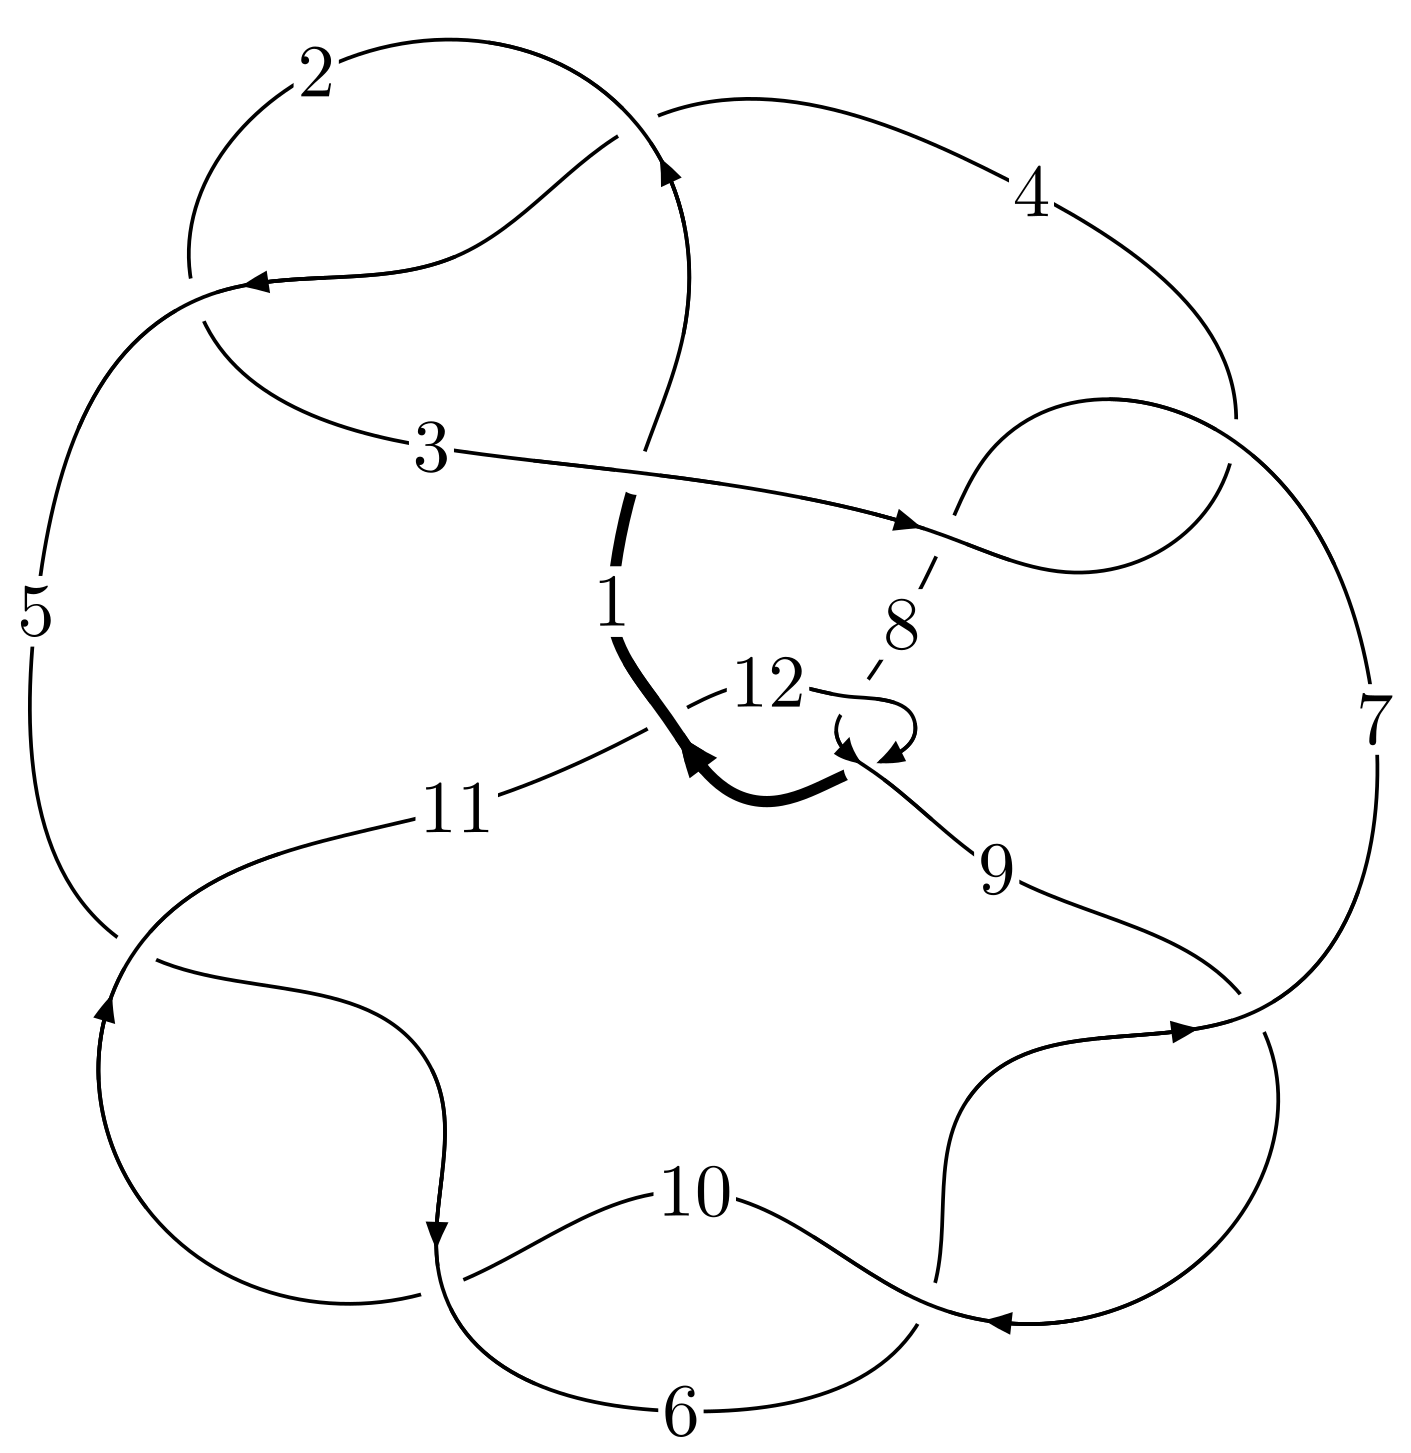
\includegraphics[width=112pt]{../../../GIT/diagram.site/Diagrams/png/2305_12n_0216.png}\\
\ \ \ A knot diagram\footnotemark}&
\allowdisplaybreaks
\textbf{Linearized knot diagam} \\
\cline{2-2}
 &
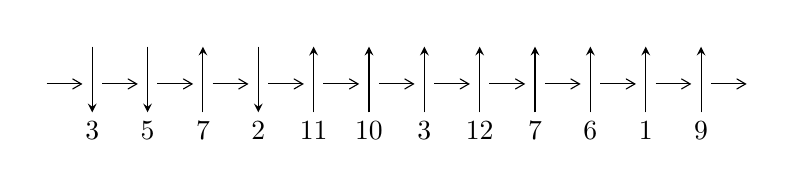
\begin{tikzpicture}[x=20pt, y=17pt]
	% nodes
	\node (C0) at (0, 0) {};
	\node (C1) at (1, 0) {};
	\node (C1U) at (1, +1) {};
	\node (C1D) at (1, -1) {3};

	\node (C2) at (2, 0) {};
	\node (C2U) at (2, +1) {};
	\node (C2D) at (2, -1) {5};

	\node (C3) at (3, 0) {};
	\node (C3U) at (3, +1) {};
	\node (C3D) at (3, -1) {7};

	\node (C4) at (4, 0) {};
	\node (C4U) at (4, +1) {};
	\node (C4D) at (4, -1) {2};

	\node (C5) at (5, 0) {};
	\node (C5U) at (5, +1) {};
	\node (C5D) at (5, -1) {11};

	\node (C6) at (6, 0) {};
	\node (C6U) at (6, +1) {};
	\node (C6D) at (6, -1) {10};

	\node (C7) at (7, 0) {};
	\node (C7U) at (7, +1) {};
	\node (C7D) at (7, -1) {3};

	\node (C8) at (8, 0) {};
	\node (C8U) at (8, +1) {};
	\node (C8D) at (8, -1) {12};

	\node (C9) at (9, 0) {};
	\node (C9U) at (9, +1) {};
	\node (C9D) at (9, -1) {7};

	\node (C10) at (10, 0) {};
	\node (C10U) at (10, +1) {};
	\node (C10D) at (10, -1) {6};

	\node (C11) at (11, 0) {};
	\node (C11U) at (11, +1) {};
	\node (C11D) at (11, -1) {1};

	\node (C12) at (12, 0) {};
	\node (C12U) at (12, +1) {};
	\node (C12D) at (12, -1) {9};
	\node (C13) at (13, 0) {};

	% arrows
	\draw[->,>={angle 60}]
	(C0) edge (C1) (C1) edge (C2) (C2) edge (C3) (C3) edge (C4) (C4) edge (C5) (C5) edge (C6) (C6) edge (C7) (C7) edge (C8) (C8) edge (C9) (C9) edge (C10) (C10) edge (C11) (C11) edge (C12) (C12) edge (C13) ;	\draw[->,>=stealth]
	(C1U) edge (C1D) (C2U) edge (C2D) (C3D) edge (C3U) (C4U) edge (C4D) (C5D) edge (C5U) (C6D) edge (C6U) (C7D) edge (C7U) (C8D) edge (C8U) (C9D) edge (C9U) (C10D) edge (C10U) (C11D) edge (C11U) (C12D) edge (C12U) ;
	\end{tikzpicture} \\
\hhline{~~} \\& 
\textbf{Solving Sequence} \\ \cline{2-2} 
 &
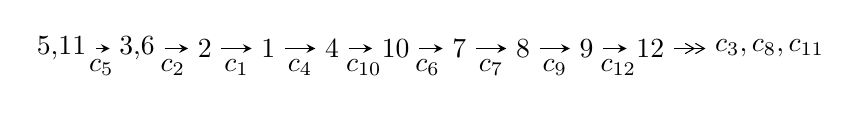
\begin{tikzpicture}[x=23pt, y=7pt]
	% node
	\node (A0) at (-1/8, 0) {5,11};
	\node (A1) at (17/16, 0) {3,6};
	\node (A2) at (17/8, 0) {2};
	\node (A3) at (25/8, 0) {1};
	\node (A4) at (33/8, 0) {4};
	\node (A5) at (41/8, 0) {10};
	\node (A6) at (49/8, 0) {7};
	\node (A7) at (57/8, 0) {8};
	\node (A8) at (65/8, 0) {9};
	\node (A9) at (73/8, 0) {12};
	\node (C1) at (1/2, -1) {$c_{5}$};
	\node (C2) at (13/8, -1) {$c_{2}$};
	\node (C3) at (21/8, -1) {$c_{1}$};
	\node (C4) at (29/8, -1) {$c_{4}$};
	\node (C5) at (37/8, -1) {$c_{10}$};
	\node (C6) at (45/8, -1) {$c_{6}$};
	\node (C7) at (53/8, -1) {$c_{7}$};
	\node (C8) at (61/8, -1) {$c_{9}$};
	\node (C9) at (69/8, -1) {$c_{12}$};
	\node (A10) at (11, 0) {$c_{3},c_{8},c_{11}$};

	% edge
	\draw[->,>=stealth]	
	(A0) edge (A1) (A1) edge (A2) (A2) edge (A3) (A3) edge (A4) (A4) edge (A5) (A5) edge (A6) (A6) edge (A7) (A7) edge (A8) (A8) edge (A9) ;
	\draw[->>,>={angle 60}]	
	(A9) edge (A10);
\end{tikzpicture} \\ 

\end{tabular} \\

\footnotetext{
The image of knot diagram is generated by the software ``\textbf{Draw programme}" developed by Andrew Bartholomew(\url{http://www.layer8.co.uk/maths/draw/index.htm\#Running-draw}), where we modified some parts for our purpose(\url{https://github.com/CATsTAILs/LinksPainter}).
}\phantom \\ \newline 
\centering \textbf{Ideals for irreducible components\footnotemark of $X_{\text{par}}$} 
 
\begin{align*}
I^u_{1}&=\langle 
-4.21983\times10^{23} u^{45}-8.41658\times10^{23} u^{44}+\cdots+1.74819\times10^{25} b+1.68172\times10^{25},\\
\phantom{I^u_{1}}&\phantom{= \langle  }5.61193\times10^{25} u^{45}+9.57494\times10^{25} u^{44}+\cdots+5.24457\times10^{25} a-1.61715\times10^{26},\;u^{46}+2 u^{45}+\cdots-2 u-1\rangle \\
I^u_{2}&=\langle 
b+1,\;-4 u^4-3 u^3-16 u^2+3 a-8 u-10,\;u^5+u^4+4 u^3+3 u^2+3 u+1\rangle \\
\\
\end{align*}
\raggedright * 2 irreducible components of $\dim_{\mathbb{C}}=0$, with total 51 representations.\\
\footnotetext{All coefficients of polynomials are rational numbers. But the coefficients are sometimes approximated in decimal forms when there is not enough margin.}
\newpage
\renewcommand{\arraystretch}{1}
\centering \section*{I. $I^u_{1}= \langle -4.22\times10^{23} u^{45}-8.42\times10^{23} u^{44}+\cdots+1.75\times10^{25} b+1.68\times10^{25},\;5.61\times10^{25} u^{45}+9.57\times10^{25} u^{44}+\cdots+5.24\times10^{25} a-1.62\times10^{26},\;u^{46}+2 u^{45}+\cdots-2 u-1 \rangle$}
\flushleft \textbf{(i) Arc colorings}\\
\begin{tabular}{m{7pt} m{180pt} m{7pt} m{180pt} }
\flushright $a_{5}=$&$\begin{pmatrix}1\\0\end{pmatrix}$ \\
\flushright $a_{11}=$&$\begin{pmatrix}0\\u\end{pmatrix}$ \\
\flushright $a_{3}=$&$\begin{pmatrix}-1.07005 u^{45}-1.82569 u^{44}+\cdots+0.723738 u+3.08347\\0.0241383 u^{45}+0.0481445 u^{44}+\cdots+0.143640 u-0.961979\end{pmatrix}$ \\
\flushright $a_{6}=$&$\begin{pmatrix}1\\- u^2\end{pmatrix}$ \\
\flushright $a_{2}=$&$\begin{pmatrix}-1.04591 u^{45}-1.77754 u^{44}+\cdots+0.867378 u+2.12149\\0.0241383 u^{45}+0.0481445 u^{44}+\cdots+0.143640 u-0.961979\end{pmatrix}$ \\
\flushright $a_{1}=$&$\begin{pmatrix}0.0994285 u^{45}+0.221105 u^{44}+\cdots+1.08052 u-0.717471\\-0.00754267 u^{45}-0.0219064 u^{44}+\cdots-0.248343 u-0.0694190\end{pmatrix}$ \\
\flushright $a_{4}=$&$\begin{pmatrix}-1.07052 u^{45}-1.81843 u^{44}+\cdots+0.520366 u+3.00463\\0.0354011 u^{45}+0.0802965 u^{44}+\cdots+0.198435 u-0.928318\end{pmatrix}$ \\
\flushright $a_{10}=$&$\begin{pmatrix}- u\\u^3+u\end{pmatrix}$ \\
\flushright $a_{7}=$&$\begin{pmatrix}u^2+1\\- u^4-2 u^2\end{pmatrix}$ \\
\flushright $a_{8}=$&$\begin{pmatrix}0.165056 u^{45}+0.387185 u^{44}+\cdots+0.706572 u-0.840882\\-0.0901646 u^{45}-0.201814 u^{44}+\cdots-0.153596 u-0.00307950\end{pmatrix}$ \\
\flushright $a_{9}=$&$\begin{pmatrix}- u^3-2 u\\u^5+3 u^3+u\end{pmatrix}$ \\
\flushright $a_{12}=$&$\begin{pmatrix}0.0405799 u^{45}+0.0527587 u^{44}+\cdots+0.527814 u-0.594467\\0.0262559 u^{45}+0.0868893 u^{44}+\cdots+0.292290 u-0.0473460\end{pmatrix}$\\&\end{tabular}
\flushleft \textbf{(ii) Obstruction class $= -1$}\\~\\
\flushleft \textbf{(iii) Cusp Shapes $= -\frac{137031846514290403395844549}{52445666902110261527019099} u^{45}-\frac{187863952688362993244773694}{52445666902110261527019099} u^{44}+\cdots-\frac{339060758282659867787462366}{52445666902110261527019099} u+\frac{588126496378574410227166340}{52445666902110261527019099}$}\\~\\
\newpage\renewcommand{\arraystretch}{1}
\flushleft \textbf{(iv) u-Polynomials at the component}\newline \\
\begin{tabular}{m{50pt}|m{274pt}}
Crossings & \hspace{64pt}u-Polynomials at each crossing \\
\hline $$\begin{aligned}c_{1}\end{aligned}$$&$\begin{aligned}
&u^{46}+18 u^{45}+\cdots+7846 u+81
\end{aligned}$\\
\hline $$\begin{aligned}c_{2},c_{4}\end{aligned}$$&$\begin{aligned}
&u^{46}-6 u^{45}+\cdots+130 u-9
\end{aligned}$\\
\hline $$\begin{aligned}c_{3},c_{7}\end{aligned}$$&$\begin{aligned}
&u^{46}-3 u^{45}+\cdots-1536 u+288
\end{aligned}$\\
\hline $$\begin{aligned}c_{5},c_{6},c_{9}\\c_{10}\end{aligned}$$&$\begin{aligned}
&u^{46}+2 u^{45}+\cdots-2 u-1
\end{aligned}$\\
\hline $$\begin{aligned}c_{8},c_{12}\end{aligned}$$&$\begin{aligned}
&u^{46}-2 u^{45}+\cdots-2 u+1
\end{aligned}$\\
\hline $$\begin{aligned}c_{11}\end{aligned}$$&$\begin{aligned}
&u^{46}-26 u^{45}+\cdots+12 u^2+1
\end{aligned}$\\
\hline
\end{tabular}\\~\\
\newpage\renewcommand{\arraystretch}{1}
\flushleft \textbf{(v) Riley Polynomials at the component}\newline \\
\begin{tabular}{m{50pt}|m{274pt}}
Crossings & \hspace{64pt}Riley Polynomials at each crossing \\
\hline $$\begin{aligned}c_{1}\end{aligned}$$&$\begin{aligned}
&y^{46}+26 y^{45}+\cdots-38928154 y+6561
\end{aligned}$\\
\hline $$\begin{aligned}c_{2},c_{4}\end{aligned}$$&$\begin{aligned}
&y^{46}-18 y^{45}+\cdots-7846 y+81
\end{aligned}$\\
\hline $$\begin{aligned}c_{3},c_{7}\end{aligned}$$&$\begin{aligned}
&y^{46}-33 y^{45}+\cdots-1930752 y+82944
\end{aligned}$\\
\hline $$\begin{aligned}c_{5},c_{6},c_{9}\\c_{10}\end{aligned}$$&$\begin{aligned}
&y^{46}+50 y^{45}+\cdots-32 y^2+1
\end{aligned}$\\
\hline $$\begin{aligned}c_{8},c_{12}\end{aligned}$$&$\begin{aligned}
&y^{46}-26 y^{45}+\cdots+12 y^2+1
\end{aligned}$\\
\hline $$\begin{aligned}c_{11}\end{aligned}$$&$\begin{aligned}
&y^{46}-10 y^{45}+\cdots+24 y+1
\end{aligned}$\\
\hline
\end{tabular}\\~\\
\newpage\flushleft \textbf{(vi) Complex Volumes and Cusp Shapes}
$$\begin{array}{c|c|c}  
\text{Solutions to }I^u_{1}& \I (\text{vol} + \sqrt{-1}CS) & \text{Cusp shape}\\
 \hline 
\begin{aligned}
u &= \phantom{-}0.259312 + 1.012880 I \\
a &= \phantom{-}0.498291 + 0.227894 I \\
b &= \phantom{-}0.517237 - 0.014608 I\end{aligned}
 & -2.49534 + 2.30202 I & \phantom{-}6.60083 - 3.93064 I \\ \hline\begin{aligned}
u &= \phantom{-}0.259312 - 1.012880 I \\
a &= \phantom{-}0.498291 - 0.227894 I \\
b &= \phantom{-}0.517237 + 0.014608 I\end{aligned}
 & -2.49534 - 2.30202 I & \phantom{-}6.60083 + 3.93064 I \\ \hline\begin{aligned}
u &= -0.710586 + 0.602137 I \\
a &= \phantom{-}0.01222 - 1.76555 I \\
b &= \phantom{-}1.154920 + 0.784082 I\end{aligned}
 & \phantom{-}4.96953 - 10.55700 I & \phantom{-}6.43149 + 8.05936 I \\ \hline\begin{aligned}
u &= -0.710586 - 0.602137 I \\
a &= \phantom{-}0.01222 + 1.76555 I \\
b &= \phantom{-}1.154920 - 0.784082 I\end{aligned}
 & \phantom{-}4.96953 + 10.55700 I & \phantom{-}6.43149 - 8.05936 I \\ \hline\begin{aligned}
u &= \phantom{-}0.675679 + 0.631174 I \\
a &= \phantom{-}0.24305 + 1.51831 I \\
b &= \phantom{-}0.978521 - 0.692213 I\end{aligned}
 & \phantom{-}1.56779 + 5.03517 I & \phantom{-}4.14094 - 5.54867 I \\ \hline\begin{aligned}
u &= \phantom{-}0.675679 - 0.631174 I \\
a &= \phantom{-}0.24305 - 1.51831 I \\
b &= \phantom{-}0.978521 + 0.692213 I\end{aligned}
 & \phantom{-}1.56779 - 5.03517 I & \phantom{-}4.14094 + 5.54867 I \\ \hline\begin{aligned}
u &= -0.758697 + 0.431488 I \\
a &= -1.026110 + 0.552682 I \\
b &= \phantom{-}1.013380 - 0.770093 I\end{aligned}
 & \phantom{-}5.47973 + 5.67003 I & \phantom{-}7.65149 - 3.29521 I \\ \hline\begin{aligned}
u &= -0.758697 - 0.431488 I \\
a &= -1.026110 - 0.552682 I \\
b &= \phantom{-}1.013380 + 0.770093 I\end{aligned}
 & \phantom{-}5.47973 - 5.67003 I & \phantom{-}7.65149 + 3.29521 I \\ \hline\begin{aligned}
u &= -0.622930 + 0.576977 I \\
a &= \phantom{-}0.72635 - 1.68752 I \\
b &= \phantom{-}0.746113 + 0.878089 I\end{aligned}
 & \phantom{-}6.32199 - 0.44657 I & \phantom{-}8.55736 + 2.63861 I \\ \hline\begin{aligned}
u &= -0.622930 - 0.576977 I \\
a &= \phantom{-}0.72635 + 1.68752 I \\
b &= \phantom{-}0.746113 - 0.878089 I\end{aligned}
 & \phantom{-}6.32199 + 0.44657 I & \phantom{-}8.55736 - 2.63861 I\\
 \hline 
 \end{array}$$\newpage$$\begin{array}{c|c|c}  
\text{Solutions to }I^u_{1}& \I (\text{vol} + \sqrt{-1}CS) & \text{Cusp shape}\\
 \hline 
\begin{aligned}
u &= \phantom{-}0.715782 + 0.374629 I \\
a &= -0.681475 - 0.671267 I \\
b &= \phantom{-}0.733462 + 0.712339 I\end{aligned}
 & \phantom{-}2.32069 - 0.37269 I & \phantom{-}6.25841 - 0.23771 I \\ \hline\begin{aligned}
u &= \phantom{-}0.715782 - 0.374629 I \\
a &= -0.681475 + 0.671267 I \\
b &= \phantom{-}0.733462 - 0.712339 I\end{aligned}
 & \phantom{-}2.32069 + 0.37269 I & \phantom{-}6.25841 + 0.23771 I \\ \hline\begin{aligned}
u &= -0.655218 + 0.438720 I \\
a &= -0.759960 + 1.146150 I \\
b &= \phantom{-}0.597845 - 1.070520 I\end{aligned}
 & \phantom{-}6.73467 - 3.88264 I & \phantom{-}9.37340 + 4.32110 I \\ \hline\begin{aligned}
u &= -0.655218 - 0.438720 I \\
a &= -0.759960 - 1.146150 I \\
b &= \phantom{-}0.597845 + 1.070520 I\end{aligned}
 & \phantom{-}6.73467 + 3.88264 I & \phantom{-}9.37340 - 4.32110 I \\ \hline\begin{aligned}
u &= \phantom{-}0.368893 + 0.464171 I \\
a &= \phantom{-}0.53754 - 1.74308 I \\
b &= -0.708048 + 0.784129 I\end{aligned}
 & \phantom{-}0.40598 + 3.67404 I & \phantom{-}5.21749 - 9.21180 I \\ \hline\begin{aligned}
u &= \phantom{-}0.368893 - 0.464171 I \\
a &= \phantom{-}0.53754 + 1.74308 I \\
b &= -0.708048 - 0.784129 I\end{aligned}
 & \phantom{-}0.40598 - 3.67404 I & \phantom{-}5.21749 + 9.21180 I \\ \hline\begin{aligned}
u &= \phantom{-}0.05290 + 1.42813 I \\
a &= \phantom{-}0.72501 - 2.48091 I \\
b &= -0.789579 + 0.086473 I\end{aligned}
 & -4.45315 + 0.20583 I & \phantom{-0.000000 } 0 \\ \hline\begin{aligned}
u &= \phantom{-}0.05290 - 1.42813 I \\
a &= \phantom{-}0.72501 + 2.48091 I \\
b &= -0.789579 - 0.086473 I\end{aligned}
 & -4.45315 - 0.20583 I & \phantom{-0.000000 } 0 \\ \hline\begin{aligned}
u &= \phantom{-}0.19161 + 1.43230 I \\
a &= -0.062200 - 0.309987 I \\
b &= \phantom{-}0.325781 + 0.842227 I\end{aligned}
 & -3.38050 + 2.83012 I & \phantom{-0.000000 } 0 \\ \hline\begin{aligned}
u &= \phantom{-}0.19161 - 1.43230 I \\
a &= -0.062200 + 0.309987 I \\
b &= \phantom{-}0.325781 - 0.842227 I\end{aligned}
 & -3.38050 - 2.83012 I & \phantom{-0.000000 } 0\\
 \hline 
 \end{array}$$\newpage$$\begin{array}{c|c|c}  
\text{Solutions to }I^u_{1}& \I (\text{vol} + \sqrt{-1}CS) & \text{Cusp shape}\\
 \hline 
\begin{aligned}
u &= -0.27356 + 1.44035 I \\
a &= -0.140805 - 0.034476 I \\
b &= \phantom{-}0.811531 - 0.701279 I\end{aligned}
 & -0.51754 + 1.93209 I & \phantom{-0.000000 } 0 \\ \hline\begin{aligned}
u &= -0.27356 - 1.44035 I \\
a &= -0.140805 + 0.034476 I \\
b &= \phantom{-}0.811531 + 0.701279 I\end{aligned}
 & -0.51754 - 1.93209 I & \phantom{-0.000000 } 0 \\ \hline\begin{aligned}
u &= -0.05653 + 1.48759 I \\
a &= -0.480692 + 0.975143 I \\
b &= -1.162780 - 0.588341 I\end{aligned}
 & -7.90348 - 1.78350 I & \phantom{-0.000000 } 0 \\ \hline\begin{aligned}
u &= -0.05653 - 1.48759 I \\
a &= -0.480692 - 0.975143 I \\
b &= -1.162780 + 0.588341 I\end{aligned}
 & -7.90348 + 1.78350 I & \phantom{-0.000000 } 0 \\ \hline\begin{aligned}
u &= -0.105822 + 0.496599 I \\
a &= \phantom{-}0.191381 + 0.934900 I \\
b &= -1.291070 - 0.220220 I\end{aligned}
 & -2.01082 - 1.28906 I & -0.35608 + 4.03643 I \\ \hline\begin{aligned}
u &= -0.105822 - 0.496599 I \\
a &= \phantom{-}0.191381 - 0.934900 I \\
b &= -1.291070 + 0.220220 I\end{aligned}
 & -2.01082 + 1.28906 I & -0.35608 - 4.03643 I \\ \hline\begin{aligned}
u &= -0.20014 + 1.48162 I \\
a &= -0.340642 + 0.355766 I \\
b &= \phantom{-}0.448756 - 1.274480 I\end{aligned}
 & \phantom{-}0.49598 - 6.93601 I & \phantom{-0.000000 } 0 \\ \hline\begin{aligned}
u &= -0.20014 - 1.48162 I \\
a &= -0.340642 - 0.355766 I \\
b &= \phantom{-}0.448756 + 1.274480 I\end{aligned}
 & \phantom{-}0.49598 + 6.93601 I & \phantom{-0.000000 } 0 \\ \hline\begin{aligned}
u &= \phantom{-}0.09377 + 1.49931 I \\
a &= -0.230681 - 0.883359 I \\
b &= -0.93270 + 1.07583 I\end{aligned}
 & -6.07967 + 5.26868 I & \phantom{-0.000000 } 0 \\ \hline\begin{aligned}
u &= \phantom{-}0.09377 - 1.49931 I \\
a &= -0.230681 + 0.883359 I \\
b &= -0.93270 - 1.07583 I\end{aligned}
 & -6.07967 - 5.26868 I & \phantom{-0.000000 } 0\\
 \hline 
 \end{array}$$\newpage$$\begin{array}{c|c|c}  
\text{Solutions to }I^u_{1}& \I (\text{vol} + \sqrt{-1}CS) & \text{Cusp shape}\\
 \hline 
\begin{aligned}
u &= -0.01965 + 1.50818 I \\
a &= -0.640464 + 0.357070 I \\
b &= -1.60059 - 0.26485 I\end{aligned}
 & -8.66214 - 1.68025 I & \phantom{-0.000000 } 0 \\ \hline\begin{aligned}
u &= -0.01965 - 1.50818 I \\
a &= -0.640464 - 0.357070 I \\
b &= -1.60059 + 0.26485 I\end{aligned}
 & -8.66214 + 1.68025 I & \phantom{-0.000000 } 0 \\ \hline\begin{aligned}
u &= \phantom{-}0.379690 + 0.276434 I \\
a &= \phantom{-}2.90356 - 0.73348 I \\
b &= -0.621326 - 0.321322 I\end{aligned}
 & \phantom{-}0.91598 - 1.09390 I & \phantom{-}7.82328 - 2.45521 I \\ \hline\begin{aligned}
u &= \phantom{-}0.379690 - 0.276434 I \\
a &= \phantom{-}2.90356 + 0.73348 I \\
b &= -0.621326 + 0.321322 I\end{aligned}
 & \phantom{-}0.91598 + 1.09390 I & \phantom{-}7.82328 + 2.45521 I \\ \hline\begin{aligned}
u &= -0.234347 + 0.374492 I \\
a &= \phantom{-}0.49536 + 2.14693 I \\
b &= -0.906115 - 0.270833 I\end{aligned}
 & -1.68679 - 0.81939 I & -2.39555 + 2.24421 I \\ \hline\begin{aligned}
u &= -0.234347 - 0.374492 I \\
a &= \phantom{-}0.49536 - 2.14693 I \\
b &= -0.906115 + 0.270833 I\end{aligned}
 & -1.68679 + 0.81939 I & -2.39555 - 2.24421 I \\ \hline\begin{aligned}
u &= -0.19365 + 1.56498 I \\
a &= \phantom{-}1.042400 - 0.850177 I \\
b &= \phantom{-}0.909015 + 0.693734 I\end{aligned}
 & -0.81497 - 3.43039 I & \phantom{-0.000000 } 0 \\ \hline\begin{aligned}
u &= -0.19365 - 1.56498 I \\
a &= \phantom{-}1.042400 + 0.850177 I \\
b &= \phantom{-}0.909015 - 0.693734 I\end{aligned}
 & -0.81497 + 3.43039 I & \phantom{-0.000000 } 0 \\ \hline\begin{aligned}
u &= -0.23754 + 1.56315 I \\
a &= \phantom{-}0.772267 - 1.161680 I \\
b &= \phantom{-}1.27662 + 0.76890 I\end{aligned}
 & -2.1712 - 14.0664 I & \phantom{-0.000000 } 0 \\ \hline\begin{aligned}
u &= -0.23754 - 1.56315 I \\
a &= \phantom{-}0.772267 + 1.161680 I \\
b &= \phantom{-}1.27662 - 0.76890 I\end{aligned}
 & -2.1712 + 14.0664 I & \phantom{-0.000000 } 0\\
 \hline 
 \end{array}$$\newpage$$\begin{array}{c|c|c}  
\text{Solutions to }I^u_{1}& \I (\text{vol} + \sqrt{-1}CS) & \text{Cusp shape}\\
 \hline 
\begin{aligned}
u &= \phantom{-}0.417366\phantom{ +0.000000I} \\
a &= \phantom{-}0.532293\phantom{ +0.000000I} \\
b &= \phantom{-}0.114066\phantom{ +0.000000I}\end{aligned}
 & \phantom{-}0.754477\phantom{ +0.000000I} & \phantom{-}13.4070\phantom{ +0.000000I} \\ \hline\begin{aligned}
u &= \phantom{-}0.22595 + 1.57656 I \\
a &= \phantom{-}0.789787 + 0.982198 I \\
b &= \phantom{-}1.160360 - 0.650256 I\end{aligned}
 & -5.75587 + 8.40053 I & \phantom{-0.000000 } 0 \\ \hline\begin{aligned}
u &= \phantom{-}0.22595 - 1.57656 I \\
a &= \phantom{-}0.789787 - 0.982198 I \\
b &= \phantom{-}1.160360 + 0.650256 I\end{aligned}
 & -5.75587 - 8.40053 I & \phantom{-0.000000 } 0 \\ \hline\begin{aligned}
u &= -0.314185\phantom{ +0.000000I} \\
a &= \phantom{-}7.82390\phantom{ +0.000000I} \\
b &= -1.08256\phantom{ +0.000000I}\end{aligned}
 & -0.443184\phantom{ +0.000000I} & \phantom{-}35.5340\phantom{ +0.000000I} \\ \hline\begin{aligned}
u &= \phantom{-}0.05348 + 1.71450 I \\
a &= \phantom{-}0.747709 + 0.114247 I \\
b &= \phantom{-}0.822911 - 0.071773 I\end{aligned}
 & -12.22280 + 3.49084 I & \phantom{-0.000000 } 0 \\ \hline\begin{aligned}
u &= \phantom{-}0.05348 - 1.71450 I \\
a &= \phantom{-}0.747709 - 0.114247 I \\
b &= \phantom{-}0.822911 + 0.071773 I\end{aligned}
 & -12.22280 - 3.49084 I & \phantom{-0.000000 } 0\\
 \hline 
 \end{array}$$\newpage\newpage\renewcommand{\arraystretch}{1}
\centering \section*{II. $I^u_{2}= \langle b+1,\;-4 u^4-3 u^3-16 u^2+3 a-8 u-10,\;u^5+u^4+4 u^3+3 u^2+3 u+1 \rangle$}
\flushleft \textbf{(i) Arc colorings}\\
\begin{tabular}{m{7pt} m{180pt} m{7pt} m{180pt} }
\flushright $a_{5}=$&$\begin{pmatrix}1\\0\end{pmatrix}$ \\
\flushright $a_{11}=$&$\begin{pmatrix}0\\u\end{pmatrix}$ \\
\flushright $a_{3}=$&$\begin{pmatrix}\frac{4}{3} u^4+u^3+\frac{16}{3} u^2+\frac{8}{3} u+\frac{10}{3}\\-1\end{pmatrix}$ \\
\flushright $a_{6}=$&$\begin{pmatrix}1\\- u^2\end{pmatrix}$ \\
\flushright $a_{2}=$&$\begin{pmatrix}\frac{4}{3} u^4+u^3+\frac{16}{3} u^2+\frac{8}{3} u+\frac{7}{3}\\-1\end{pmatrix}$ \\
\flushright $a_{1}=$&$\begin{pmatrix}-1\\0\end{pmatrix}$ \\
\flushright $a_{4}=$&$\begin{pmatrix}\frac{4}{3} u^4+u^3+\frac{16}{3} u^2+\frac{8}{3} u+\frac{10}{3}\\-1\end{pmatrix}$ \\
\flushright $a_{10}=$&$\begin{pmatrix}- u\\u^3+u\end{pmatrix}$ \\
\flushright $a_{7}=$&$\begin{pmatrix}u^2+1\\- u^4-2 u^2\end{pmatrix}$ \\
\flushright $a_{8}=$&$\begin{pmatrix}u^2+1\\- u^4-2 u^2\end{pmatrix}$ \\
\flushright $a_{9}=$&$\begin{pmatrix}- u^3-2 u\\- u^4- u^3-3 u^2-2 u-1\end{pmatrix}$ \\
\flushright $a_{12}=$&$\begin{pmatrix}u\\u\end{pmatrix}$\\&\end{tabular}
\flushleft \textbf{(ii) Obstruction class $= 1$}\\~\\
\flushleft \textbf{(iii) Cusp Shapes $= \frac{14}{9} u^4+\frac{11}{3} u^3+\frac{77}{9} u^2+\frac{88}{9} u+\frac{29}{9}$}\\~\\
\newpage\renewcommand{\arraystretch}{1}
\flushleft \textbf{(iv) u-Polynomials at the component}\newline \\
\begin{tabular}{m{50pt}|m{274pt}}
Crossings & \hspace{64pt}u-Polynomials at each crossing \\
\hline $$\begin{aligned}c_{1},c_{2}\end{aligned}$$&$\begin{aligned}
&(u-1)^5
\end{aligned}$\\
\hline $$\begin{aligned}c_{3},c_{7}\end{aligned}$$&$\begin{aligned}
&u^5
\end{aligned}$\\
\hline $$\begin{aligned}c_{4}\end{aligned}$$&$\begin{aligned}
&(u+1)^5
\end{aligned}$\\
\hline $$\begin{aligned}c_{5},c_{6},c_{11}\end{aligned}$$&$\begin{aligned}
&u^5+u^4+4 u^3+3 u^2+3 u+1
\end{aligned}$\\
\hline $$\begin{aligned}c_{8}\end{aligned}$$&$\begin{aligned}
&u^5+u^4- u^2+u+1
\end{aligned}$\\
\hline $$\begin{aligned}c_{9},c_{10}\end{aligned}$$&$\begin{aligned}
&u^5- u^4+4 u^3-3 u^2+3 u-1
\end{aligned}$\\
\hline $$\begin{aligned}c_{12}\end{aligned}$$&$\begin{aligned}
&u^5- u^4+u^2+u-1
\end{aligned}$\\
\hline
\end{tabular}\\~\\
\newpage\renewcommand{\arraystretch}{1}
\flushleft \textbf{(v) Riley Polynomials at the component}\newline \\
\begin{tabular}{m{50pt}|m{274pt}}
Crossings & \hspace{64pt}Riley Polynomials at each crossing \\
\hline $$\begin{aligned}c_{1},c_{2},c_{4}\end{aligned}$$&$\begin{aligned}
&(y-1)^5
\end{aligned}$\\
\hline $$\begin{aligned}c_{3},c_{7}\end{aligned}$$&$\begin{aligned}
&y^5
\end{aligned}$\\
\hline $$\begin{aligned}c_{5},c_{6},c_{9}\\c_{10},c_{11}\end{aligned}$$&$\begin{aligned}
&y^5+7 y^4+16 y^3+13 y^2+3 y-1
\end{aligned}$\\
\hline $$\begin{aligned}c_{8},c_{12}\end{aligned}$$&$\begin{aligned}
&y^5- y^4+4 y^3-3 y^2+3 y-1
\end{aligned}$\\
\hline
\end{tabular}\\~\\
\newpage\flushleft \textbf{(vi) Complex Volumes and Cusp Shapes}
$$\begin{array}{c|c|c}  
\text{Solutions to }I^u_{2}& \I (\text{vol} + \sqrt{-1}CS) & \text{Cusp shape}\\
 \hline 
\begin{aligned}
u &= -0.233677 + 0.885557 I \\
a &= -0.162657 + 0.410020 I \\
b &= -1.00000\phantom{ +0.000000I}\end{aligned}
 & -3.46474 - 2.21397 I & -2.77420 + 4.04289 I \\ \hline\begin{aligned}
u &= -0.233677 - 0.885557 I \\
a &= -0.162657 - 0.410020 I \\
b &= -1.00000\phantom{ +0.000000I}\end{aligned}
 & -3.46474 + 2.21397 I & -2.77420 - 4.04289 I \\ \hline\begin{aligned}
u &= -0.416284\phantom{ +0.000000I} \\
a &= \phantom{-}3.11537\phantom{ +0.000000I} \\
b &= -1.00000\phantom{ +0.000000I}\end{aligned}
 & -0.762751\phantom{ +0.000000I} & \phantom{-}0.416710\phantom{ +0.000000I} \\ \hline\begin{aligned}
u &= -0.05818 + 1.69128 I \\
a &= -0.728361 + 0.139255 I \\
b &= -1.00000\phantom{ +0.000000I}\end{aligned}
 & -12.60320 - 3.33174 I & -7.32304 - 1.07305 I \\ \hline\begin{aligned}
u &= -0.05818 - 1.69128 I \\
a &= -0.728361 - 0.139255 I \\
b &= -1.00000\phantom{ +0.000000I}\end{aligned}
 & -12.60320 + 3.33174 I & -7.32304 + 1.07305 I\\
 \hline 
 \end{array}$$\newpage
\newpage\renewcommand{\arraystretch}{1}
\centering \section*{ III. u-Polynomials}
\begin{tabular}{m{50pt}|m{274pt}}
Crossings & \hspace{64pt}u-Polynomials at each crossing \\
\hline $$\begin{aligned}c_{1}\end{aligned}$$&$\begin{aligned}
&((u-1)^5)(u^{46}+18 u^{45}+\cdots+7846 u+81)
\end{aligned}$\\
\hline $$\begin{aligned}c_{2}\end{aligned}$$&$\begin{aligned}
&((u-1)^5)(u^{46}-6 u^{45}+\cdots+130 u-9)
\end{aligned}$\\
\hline $$\begin{aligned}c_{3},c_{7}\end{aligned}$$&$\begin{aligned}
&u^5(u^{46}-3 u^{45}+\cdots-1536 u+288)
\end{aligned}$\\
\hline $$\begin{aligned}c_{4}\end{aligned}$$&$\begin{aligned}
&((u+1)^5)(u^{46}-6 u^{45}+\cdots+130 u-9)
\end{aligned}$\\
\hline $$\begin{aligned}c_{5},c_{6}\end{aligned}$$&$\begin{aligned}
&(u^5+u^4+4 u^3+3 u^2+3 u+1)(u^{46}+2 u^{45}+\cdots-2 u-1)
\end{aligned}$\\
\hline $$\begin{aligned}c_{8}\end{aligned}$$&$\begin{aligned}
&(u^5+u^4- u^2+u+1)(u^{46}-2 u^{45}+\cdots-2 u+1)
\end{aligned}$\\
\hline $$\begin{aligned}c_{9},c_{10}\end{aligned}$$&$\begin{aligned}
&(u^5- u^4+4 u^3-3 u^2+3 u-1)(u^{46}+2 u^{45}+\cdots-2 u-1)
\end{aligned}$\\
\hline $$\begin{aligned}c_{11}\end{aligned}$$&$\begin{aligned}
&(u^5+u^4+4 u^3+3 u^2+3 u+1)(u^{46}-26 u^{45}+\cdots+12 u^2+1)
\end{aligned}$\\
\hline $$\begin{aligned}c_{12}\end{aligned}$$&$\begin{aligned}
&(u^5- u^4+u^2+u-1)(u^{46}-2 u^{45}+\cdots-2 u+1)
\end{aligned}$\\
\hline
\end{tabular}\newpage\renewcommand{\arraystretch}{1}
\centering \section*{ IV. Riley Polynomials}
\begin{tabular}{m{50pt}|m{274pt}}
Crossings & \hspace{64pt}Riley Polynomials at each crossing \\
\hline $$\begin{aligned}c_{1}\end{aligned}$$&$\begin{aligned}
&((y-1)^5)(y^{46}+26 y^{45}+\cdots-38928154 y+6561)
\end{aligned}$\\
\hline $$\begin{aligned}c_{2},c_{4}\end{aligned}$$&$\begin{aligned}
&((y-1)^5)(y^{46}-18 y^{45}+\cdots-7846 y+81)
\end{aligned}$\\
\hline $$\begin{aligned}c_{3},c_{7}\end{aligned}$$&$\begin{aligned}
&y^5(y^{46}-33 y^{45}+\cdots-1930752 y+82944)
\end{aligned}$\\
\hline $$\begin{aligned}c_{5},c_{6},c_{9}\\c_{10}\end{aligned}$$&$\begin{aligned}
&(y^5+7 y^4+16 y^3+13 y^2+3 y-1)(y^{46}+50 y^{45}+\cdots-32 y^2+1)
\end{aligned}$\\
\hline $$\begin{aligned}c_{8},c_{12}\end{aligned}$$&$\begin{aligned}
&(y^5- y^4+4 y^3-3 y^2+3 y-1)(y^{46}-26 y^{45}+\cdots+12 y^2+1)
\end{aligned}$\\
\hline $$\begin{aligned}c_{11}\end{aligned}$$&$\begin{aligned}
&(y^5+7 y^4+16 y^3+13 y^2+3 y-1)(y^{46}-10 y^{45}+\cdots+24 y+1)
\end{aligned}$\\
\hline
\end{tabular}
\vskip 2pc
\end{document}